\documentclass[12pt]{amsart}
      % \newif\ifpreview
      % \previewfalse

% approx iid
\newcommand\simiid{\stackrel{\mathclap{\normalfont\mbox{\tiny{iid}}}}{\sim}}
\usepackage{natbib}
\usepackage{titlecaps}
\Addlcwords{a about above after again against all am an and any are aren't as at be because been before being below between both but by can't cannot could couldn't did didn't do does doesn't doing don't down during each few for from further had hadn't has hasn't have haven't having he he'd he'll he's her here here's hers herself him himself his how how's i i'd i'll i'm i've if in into is isn't it it's its itself let's me more most mustn't my myself no nor not of off on once only or other ought our ours ourselves out over own same shan't she she'd she'll she's should shouldn't so some such than that that's the their theirs them themselves then there there's these they they'd they'll they're they've this those through to too under until up very was wasn't we we'd we'll we're we've were weren't what what's when when's where where's which while who who's whom why why's with won't would wouldn't you you'd you'll you're you've your yours yourself yourselves}

% Fonts
% at some point figure out bolding ...
\usepackage[default,oldstyle,scale=0.95]{opensans}
%\usepackage[sfdefault,scaled=.85]{FiraSans}
\usepackage[T1]{fontenc}
\usepackage{textcomp}
\usepackage[varqu,varl]{zi4}% inconsolata typewriter
\usepackage{amsmath,amsthm}
\usepackage[cmintegrals]{newtxsf}
\usepackage[T1]{fontenc}
\usepackage{ae}

% easy commands for number propers
\newcommand{\first}{1$^{\text{st}}$}
\newcommand{\second}{2$^{\text{nd}}$}
\newcommand{\third}{3$^{\text{rd}}$}
\newcommand{\nth}[1]{${#1}^{\text{th}}$}

% Generate some fake text
\usepackage{blindtext}

% % add watermark
% \usepackage{draftwatermark}
% \SetWatermarkText{Submission Copy}
% \SetWatermarkScale{.5}
% \SetWatermarkColor[gray]{0.9}

% layout control
\usepackage{geometry}
\geometry{verbose,tmargin=1in,bmargin=1.25in,lmargin=1in,rmargin=1in}
\usepackage{parallel}
\usepackage{parcolumns}
\usepackage{fancyhdr}
\usepackage[export]{adjustbox}
\usepackage{etoolbox}

% math typesetting
\usepackage{array}
\usepackage{amsmath}
\usepackage{amssymb}
\usepackage{amsthm}
\usepackage{amsfonts}
\usepackage{relsize}
\usepackage{mathtools}
\usepackage{bm}
%\usepackage[%decimalsymbol=.,digitsep=fullstop]{siunitx}

% restricts float objects to be inserted before end of section
% creates float barriers
\usepackage[section]{placeins}

% tables
\usepackage{tabularx}
\usepackage{booktabs}
\usepackage{multicol}
\usepackage{multirow}
\usepackage{longtable}

% to adapt caption style
\usepackage[font={small},labelfont=bf]{caption}

% footnotes at bottom
%\usepackage[bottom]{footmisc}

% to change enumeration symbols begin{enumerate}[(a)]
\usepackage{enumerate}
\usepackage{paralist}

% to colorize links in document. See color specification below
\usepackage[pdftex,hyperref,x11names]{xcolor}

% for multiple references and insertion of the word "figure" or "table"
% \usepackage{cleveref}

% load the hyper-references package and set document info
\usepackage[pdftex]{hyperref}

% graphics stuff
\usepackage{subfigure}
\usepackage{graphicx}
\usepackage[space]{grffile} % allows us to specify directories that have spaces
\usepackage{placeins} % prevents floats from moving past a \FloatBarrier
\usepackage{tikz}

% sideway figures
\usepackage{rotating}
\usepackage{lscape}

%\usepackage[figuresright]{rotating}
% \newenvironment{amssidewaysfigure}  {\begin{sidewaysfigure}\vspace*{.8\textwidth}\begin{minipage}{\textheight}\centering}
%   {\end{minipage}\end{sidewaysfigure}}

% Spacing
\usepackage[doublespacing]{setspace}

% outside code
\usepackage{listings}
\usepackage{enumitem}

% define clickable links and their colors
\hypersetup{%
	unicode=false,          % non-Latin characters in Acrobat's bookmarks
	pdftoolbar=true,        % show Acrobat's toolbar?
	pdfmenubar=true,        % show Acrobat's menu?
	pdffitwindow=false,     % window fit to page when opened
	pdfstartview={FitH},    % fits the width of the page to the window
	pdfnewwindow=true,%
	%pagebackref=false,%
	pdfauthor={Shahryar Minhas, et alia.},%
	pdftitle={Taking Dyads Seriously},%
	colorlinks,%
	citecolor=black,%
	filecolor=black,%
	linkcolor=black,%
	urlcolor=RoyalBlue4
}

% -------------------- title -------------------- %

\title{Taking Dyads Seriously}
\vspace{\baselineskip}

% \author[Minhas]{Shahryar Minhas}
% \address{Shahryar Minhas: Department of Political Science}
% \curraddr{Michigan State University}
% \email[Corresponding author]{minhassh@msu.edu}

% \author[Dorff]{Cassy L. Dorff}
% \address{Cassy L. Dorff}
% \curraddr{Department of Political Science, University of New Mexico}
% \email{cdorff@unm.edu}

% \author[Foster]{Margaret Foster}
% \address{Margaret Foster}
% \curraddr{Department of Political Science, Duke University}
% \email{margaret.foster@duke.edu}

% \author[Gallop]{Max Gallop}
% \address{Max Gallop}
% \curraddr{Department of Government and Public Policy, University of Strathclyde}
% \email{max.gallop@strath.ac.uk}

% \author[Liu]{Howard Liu}
% \address{Howard Liu}
% \curraddr{Department of Political Science, Duke University}
% \email{hao.liu@duke.edu}

% \author[Tellez]{Juan Tellez}
% \address{Juan Tellez}
% \curraddr{Department of Political Science, Duke University}
% \email{juan.tellez@duke.edu}

% \author[Ward]{Michael D. Ward}
% \address{Michael D. Ward}
% \curraddr{Department of Political Science, Duke University}
% \email{michael.d.ward@duke.edu}

% \date{\today}

% \thanks{Shahryar Minhas and Michael D. Ward acknowledge support from National Science Foundation (NSF) Award 1259266. Peter Hoff, John Ahlquist, Robert Franzese, Arturas Rozenas, Betsy Sinclair, Jacob Montgomery and Benjamin Appel provided welcome and helpful comments. We also thank Douglas Gibler for kindly providing us with a copy of the data and programs he used in \citet{gibler:2017}. We benefited from presentations of this material at the 2017 Political Methodology Conference, and our home institutions.}

\setlength{\headheight}{15pt}
\setlength{\headsep}{20pt}
\pagestyle{fancyplain}
\fancyhf{}
\lhead{\fancyplain{}{}}
% \chead{\fancyplain{}{Taking Dyads Seriously}}
\chead{\fancyplain{}{}}
% \rhead{\fancyplain{}{\today}}
\rhead{\fancyplain{}{}}
\rfoot{\fancyplain{}{\thepage}}

% references to graphics
\makeatletter
% \def\input@path{{/Users/janus829/Dropbox/toDo_notes/nsfSumm/Graphics/}, {/Users/s7m/Dropbox/toDo_notes/nsfSumm/Graphics/}}
% \graphicspath{{/Users/janus829/Dropbox/toDo_notes/nsfSumm/Graphics/}, {/Users/s7m/Dropbox/toDo_notes/nsfSumm/Graphics/}}

% easy command for boldface math symbols
\newcommand{\mbs}[1]{\boldsymbol{#1}}

% command for R package font
\newcommand{\pkg}[1]{{\fontseries{b}\selectfont #1}}

% Add some colors
\definecolor{red1}{RGB}{253,219,199}
\definecolor{red2}{RGB}{244,165,130}
\definecolor{red3}{RGB}{178,24,43}

\definecolor{green1}{RGB}{229,245,224}
\definecolor{green2}{RGB}{161,217,155}
\definecolor{green3}{RGB}{49,163,84}

\definecolor{blue0}{RGB}{255,247,251}
\definecolor{blue1}{RGB}{222,235,247}
\definecolor{blue2}{RGB}{158,202,225}
\definecolor{blue3}{RGB}{49,130,189}
\definecolor{blue4}{RGB}{4,90,141}

\definecolor{purple1}{RGB}{191,211,230}
\definecolor{purple2}{RGB}{140,150,198}
\definecolor{purple3}{RGB}{140,107,177}

\definecolor{brown1}{RGB}{246,232,195}
\definecolor{brown2}{RGB}{223,194,125}
\definecolor{brown3}{RGB}{191,129,45}

% square bracket matrices
\let\bbordermatrix\bordermatrix
\patchcmd{\bbordermatrix}{8.75}{4.75}{}{}
\patchcmd{\bbordermatrix}{\left(}{\left[}{}{}
\patchcmd{\bbordermatrix}{\right)}{\right]}{}{}


\begin{document}
% \ifpreview {
%    \definecolor{personal}{rgb}{1.0, 1.0, 0.0}
%    \pagecolor{personal}
%    }
% \fi


\small{\singlespacing{
\begin{abstract}
	International relations scholarship concerns dyads, yet standard modeling approaches fail to adequately capture the data generating process behind dyadic events and processes. As a result, they suffer from biased coefficients and poorly calibrated standard errors. We show how a regression-based approach, the Additive and Multiplicative Effects (AME) model, can be used to account for the inherent dependencies in dyadic data and glean substantive insights in the interrelations between actors. First, we conduct a simulation to highlight how the model captures dependencies and show that accounting for these processes improves our ability to conduct inference on dyadic data. Second, we compare the AME model to approaches used in three prominent studies from recent international relations scholarship. For each study, we find that compared to AME, the modeling approach used performs notably worse at capturing the data generating process. Further, conventional methods misstate the effect of key variables and the uncertainty in these effects. Finally, AME outperforms standard approaches in terms of out-of-sample fit. In sum, our work shows the consequences of failing to take the dependencies inherent to dyadic data seriously. Most importantly, by better modeling the data generating process underlying political phenomena, the AME framework improves scholars' ability to conduct inferential analyses on dyadic data.
\end{abstract}
}}


\maketitle

\begin{center}
	\textbf{Word count}: 9,542
\end{center}

\thispagestyle{empty}
\newpage\setcounter{page}{1}


\section{\textbf{Introduction}}

The aim of this study is to address how to estimate regression coefficients in a generalized linear model (GLM) context when there are network dependencies in dyadic data. Specifically, we discuss and evaluate how well the Additive and Multiplicative Effects (AME) model can be used to account for the interdependencies underlying the data generating process of dyadic structures \citep{hoff:2005,hoff:2008,minhas:etal:2019} in International Relations data. The AME works by including a set of parameters meant to capture network effects in the conditional mean equation of the GLM.

We focus on three types of network effects that can complicate dyadic analyses. First, dependencies may arise within a set of dyads if a particular actor is more likely to send or receive actions such as conflict.\footnote{In the case of undirected data where there is no clear sender or receiver, it is still essential to take into account the variance in how active actors are in the system.} Additionally, if the event of interest has a clear sender and receiver, we are likely to observe dependencies within a dyad; for example, if a rebel group initiates a conflict against a government, the government will likely reciprocate that behavior. We capture these effects, often referred to as first- and second-order dependencies, respectively, within the additive effects portion of the model. Third-order dependencies capture relationships of transitivity, balance, and clusterability between different dyads. For example, we can only understand why Poland was involved in a dyadic conflict with Iraq in 2003 if we understand that the United States invaded Iraq in 2003 and that Poland often participates in US-led coalitions. The multiplicative effects capture these sorts of dependencies, specifically, those that result because the specified model has not accounted for a latent set of shared attributes that affect actors' probability of interacting with one another.

We begin with a discussion of these dependencies and an introduction to the AME model. Next, we conduct a simulation study to show how the AME approach can recover unbiased and well-calibrated regression coefficients in the presence of network based dependence. Last, to highlight the utility of this approach, we apply the AME model to three recent studies in the international relations (IR) literature. Our comparison reveals that accounting for observational dependence leads to results that, at times, differ from those found in the original study as well as from the broader literature. Moreover, we demonstrate that the additional parameters included by AME in the conditional mean equation of a typical GLM can offer substantive insights that are often occluded by ignoring the interdependencies found in relational data. Finally, we show that for each replication our network-based approach provides substantially more accurate out-of-sample predictions than the models used in the original studies.

The AME approach advances statistical analysis of dyadic data by accounting for observational dependence while allowing scholars to test the substantive effect of variables of interest. Thus, the AME allows scholars to achieve a two-fold goal: to continue to generate meaningful, substantive insights about political phenomena without abandoning a regression based approach, while at the same time accounting for the data generating processes behind such events of interest. Perhaps most importantly, the AME approach concentrates on the relational aspect of international relations through a statistical framework that is familiar to most scholars.


\section{\textbf{Dependencies in Dyadic Data}}

When modeling dyadic data, scholars typically employ a GLM estimated via maximum-likelihood. This type of model is expressed via a stochastic and systematic component \citep{pawitan:2013}. The stochastic component reflects our assumptions about the probability distribution from which the data are generated: $y_{ij} \sim P(Y | \theta_{ij})$, with a probability density or mass function, such as the normal, binomial, or Poisson, and we assume that each dyad in the sample is independently drawn from that particular distribution, given $\theta_{ij}$. The systematic component characterizes the model for the parameters of that distribution and describes how $\theta_{ij}$ varies as a function of a set of nodal and dyadic covariatse, $\mathbf{X_{ij}}$: $\theta_{ij} = \bm\beta^{T} \mathbf{X}_{ij}$. A fundamental assumption we make when applying this modeling technique is that given $\mathbf{X}_{ij}$ and the parameters of our distribution, each of the dyadic observations are conditionally independent. The importance of this assumption becomes clearer in the process of estimating a GLM via maximum likelihood. After having chosen a set of covariates and specifying a distribution, we construct the joint density function over all dyads, for example:

\vspace{-8mm}
\begin{align}
\begin{aligned}
	P(y_{ij}, y_{ik}, \ldots | \theta_{ij}, \theta_{ik}, \ldots ) &= P(y_{ij} | \theta_{ij}) \times P(y_{ik} | \theta_{ik}) \times \ldots  \\
	P(\mathbf{Y} \; | \; \bm{\theta}) &= \prod_{\alpha=1}^{n \times (n-1)} P(y_{\alpha} | \theta_{\alpha})  \\
\end{aligned}
\end{align}

\noindent We next convert the joint probability into a likelihood: $\displaystyle \mathcal{L} (\bm{\theta} | \mathbf{Y}) = \prod_{\alpha=1}^{n \times (n-1)} P(y_{\alpha} | \theta_{\alpha})$.

We can then estimate the parameters by maximizing the likelihood, or, more typically, the log-likelihood. However, the likelihood as defined above is only valid if we are able to make the assumption that, for example, $y_{ij}$ is independent of $y_{ji}$ and $y_{ik}$ given the set of covariates we specified, or the values of $\theta_{ij}$. Without the assumption of conditional observational independence the joint density function cannot be written in the way described above and a valid likelihood does not exist. Accordingly, inferences drawn from misspecified models that ignore potential interdependencies between dyadic observations are likely to have a number of issues, including biased estimates of the effect of independent variables, uncalibrated confidence intervals, and poor predictive performance. The importance of accounting for the underlying structure of our data has been a lesson well understood, at least when it comes to time-series cross-sectional data (TSCS) within political science \citep{beck:katz:1995,beck:etal:1998}. As a result, it is now standard practice to take explicit steps to account for the complex data structures that emerge in TSCS applications and the unobserved heterogeneity that they cause.

% Scholars working with dyadic data typically begin by stacking observations associated with each dyad on top of one another and not passing any auxiliary information to the model about how observations may be interdependent. For example, in this design, a conflict initiated from the United States against Japan is assumed to be independent of any conflictual action that Japan may send to the United States. Additionally, every action sent by Japan to others in the system is considered independent even though each of those interactions involves a common sender, i.e, Japan. While most scholars begin with the assumption that each dyadic interaction takes place in isolation of the others, we know this assumption to be false both in theory and in practice. Relational data comes with an explicit structure that generally leads to particular types of dependencies. The importance of accounting for the underlying structure of our data has been a lesson well understood, at least when it comes to time-series cross-sectional data (TSCS) within political science \citep{beck:katz:1995,beck:etal:1998}. As a result, it is now standard practice to take explicit steps to account for the complex data structures that emerge in TSCS applications and the unobserved heterogeneity that they cause.

To uncover the underlying structure of relational data, it is helpful to restructure dyadic data in the form of a matrix---often referred to as an adjacency matrix---as shown in Figure~\ref{fig:adjMatDeps}. Rows designate the senders of an event and columns the receivers. The cross-sections in this matrix represent the actions that were sent by an actor in the row to those designated in the columns. Thus $y_{ij}$ designates an action $y$, such as a conflictual event or trade flow, that is sent from actor $i$ to actor $j$. In many applications, scholars are interested in studying undirected (i.e., symmetric) outcomes in which there is no clear sender or receiver, these type of outcomes still can, and we argue should, be studied using the type of framework we discuss below.

Using the structure of an adjacency matrix, Figure~\ref{fig:adjMatDeps} visualizes the types of first- and second-order dependencies that can complicate the analysis of relational data in traditional GLMs. The adjacency matrix on the top left highlights a particular row to illustrate that these values may be more similar to each other than other values because each has a common sender. Interactions involving a common sender also manifest heterogeneity in how active actors are across the network when compared to each other. In most relational datasets (e.g., trade flows, conflict, participation in international organizations, even networks derived from Twitter or Facebook), we often find that there are some actors that are much more active than others \citep{barabasi:reka:1999}. For example, in an analysis of international trade certain countries (e.g., China) export much larger volumes than other countries for a variety of structural, contextual, and idiosyncratic reasons. Unless one is able to develop a model that can account for the variety of explanations that may play a role in determining why a particular actor is more active than others, parameter estimates from standard statistical models will be biased.\footnote{In an undirected setting instead of studying sender and receiver heterogeneity, we would just be concerned with actor heterogeneity in general.}

\begin{figure}
	\begin{tabular}{cc}
		\textsc{Sender Heterogeneity} & \textsc{Receiver Heterogeneity} \\
		\includegraphics[width=.4\textwidth]{graphics/adjRowDep.png} &
		\includegraphics[width=.4\textwidth]{graphics/adjColDep.png} \\
		\textsc{Sender-Receiver Covariance} & \textsc{Reciprocity} \\
		\includegraphics[width=.4\textwidth]{graphics/adjRowColCovar.png} &
		\includegraphics[width=.4\textwidth]{graphics/adjRecip.png} \\
	\end{tabular}
	\caption{Nodal and dyadic dependencies in relational data.}
	\label{fig:adjMatDeps}
\end{figure}

For similar reasons one also needs to take into account the dependence between observations that share a common receiver. The bottom-left panel in Figure~\ref{fig:adjMatDeps} illustrates that sender and receiver type dependencies can also blend together. Specifically, actors who are more likely to send ties in a network tend to also be more likely to receive them. As a result, the rows and columns in an adjacency matrix are often correlated. For example, consider trade flows both from and to many wealthy, developed countries. The bottom-right panel highlights a second-order dependence, specifically, reciprocity. This is a dependency occurring within dyads involving the same actors whereby values of $y_{ij}$ and $y_{ji}$ are correlated. The concept of reciprocity has deep roots in the study of relations between states \citep{richardson:1960,keohane:1989}.

For most relational data, however, dependencies do not simply manifest at the nodal or dyadic level. More often we find significant evidence of higher-order structures that result from dependencies between multiple groups of actors. These dependencies arise because there may be a set of latent attributes between actors that affects their probability of interacting with one another \citep{zinnes:1967,wasserman:faust:1994}. In Figure~\ref{fig:thirdDeps} we provide a visualization of a simulated relational dataset wherein the nodes designate actors and edges between the nodes indicate that an interaction between the two took place. To highlight third-order dependence patterns, nodes with similar latent attributes are colored similarly.

\begin{figure}[ht]
	\includegraphics[width=.6\textwidth]{graphics/stochEquiv_v2.pdf}
	\caption{Higher-order dependence patterns in a network.}
	% need a simpler caption here
	\label{fig:thirdDeps}
\end{figure}

The visualization illustrates that actors belonging to the same group have a higher likelihood of interacting with each other, whereas interactions across groups are rarer. A prominent example of a network with this type of structure is discussed by \citet{adamic:glance:2005}, who visualize linkages between political blogs preceding the 2004 United States Presidential Election. \citeauthor{adamic:glance:2005} find that the degree of interaction between right- and left-leaning blogs is minimal and that most blogs are linked to others that are politically similar. This showcases the types of higher-order dependencies that can emerge in relational data. First, the fact that interactions are determined by a shared attribute, in this case political ideology, is an example of \textit{homophily}. Homophily explains the emergence of patterns such as transitivity (``a friend of a friend is a friend'') and balance (``an enemy of a friend is an enemy''), which also have a long history in international relations. The other major type of meso-scopic features that emerge in relational data is community structure \citep{mucha:etal:2010}, which is often formalized through the concept of stochastic equivalence \citep{anderson:etal:1992}. Stochastic equivalence refers to a type of pattern in which actors can be divided into groups such that members of the same group have similar patterns of relationships. In the example above, each of the left leaning blogs would be considered stochastically equivalent to one another because any given left-leaning blog is more likely to interact with a blog of a similar political position and less likely to interact with one of a divergent political position.

These types of patterns frequently emerge in IR contexts.\footnote{For example, see: \citet{manger:etal:2012, kinne:2013, chyzh:2016}.} For example, a perennial finding in the interstate trade literature emphasizes the role that geography plays in determining trade flows. Geographic proximity in the network context is an example of homophily---a shared attribute between actors that corresponds to a greater likelihood of the event of interest taking place. Alternatively, in the interstate conflict literature, we may find that actors who are each a member of a particular (formal or informal) alliance are likely to act similarly in the conflict network. Specifically, they will tend to initiate conflictual events with actors that their fellow alliance members initiate conflict with, and they will be unlikely to initiate conflict with members of their alliance---an example of stochastic equivalence. In both these examples, we are able to explicitly parameterize the attribute that might explain the emergence of higher order dependence patterns. While sometimes the conditions driving these patterns, such as geography, are easy to identify, at other times it can be difficult to describe exactly why higher order dependence patterns in networks may develop.

% International Trade, we might observe homophily wherein states with open economies and an absence of Non-Tariff Barriers are more likely to trade with each-other all else equal; alternatively we might observe heterophily in the sense that states that have greater endowments of capital are more likely to trade with states with greater endowments of land or labor.

%  We would also likely observe stochastic equivalence in an interstate war network wherein countries who are in conflict with the same target country are unlikely to fight one another. In this case, countries with (formal or informal) alliances are a member of the same group due to similar conflictual ties to other actors in the system.

\section{\textbf{Additive and Multiplicative Effect Models for Networks}}

To account for the dependencies that are prevalent in dyadic data, we turn to the AME model. The AME approach can be used to conduct inference on cross-sectional and longitudinal networks with binary, ordinal, or continuous linkages. It is flexible and easy to use for analyzing the kind of relational data often found in the social sciences. It accounts for nodal and dyadic dependence patterns, as well as higher-order dependencies such as homophily and stochastic equivalence.\footnote{\citet{minhas:etal:2019} detail how this framework contrasts with alternative network-based approaches. } The AME model combines the social relations regression model (SRRM) to account for nodal and dyadic dependencies and the latent factor model (LFM) for third-order dependencies.\footnote{An earlier version of the LFM  used in AME is presented as the general bilinear mixed effects (GBME) model in \citet{hoff:2005}. The GBME model is more limited in the types of dependence patterns that it can capture due to the formulation of the matrix decomposition procedure.}  For details on the SRRM see \citet{li:loken:2002,hoff:2005,dorff:minhas:2017}. The AME model is specified as follows:

\begin{align}
	\begin{aligned}
		y_{ij} \;=\; f(\theta_{ij}) &\text{, where } \\
		\theta_{ij} \;=\;& \bm\beta_{d}^{\top} \mathbf{X}_{ij} + \bm\beta_{s}^{\top} \mathbf{X}_{i} + \bm\beta_{r}^{\top} \mathbf{X}_{j} \text{\qquad(Exogenous parameters)} \\
		& + a_{i} + b_{j} + \epsilon_{ij} \text{\qquad\qquad\qquad\quad(SRRM parameters)} \\
		& + \mathbf{u}_{i}^{\top} \mathbf{D} \mathbf{v}_{j}  \text{\qquad\qquad\qquad\qquad\qquad\;(LFM parameters)} \\
	\label{eqn:ame}
	\end{aligned}
\end{align}

% We use a Bayesian probit framework, in which we model a latent variable, $\theta_{ij}$, first using a set of exogenous dyadic ($\bm\beta_{d}^{\top} \mathbf{X}_{ij}$), sender ($\bm\beta_{s}^{\top} \mathbf{X}_{i}$), and receiver covariates ($\bm\beta_{r}^{\top} \mathbf{X}_{j}$).
where $y_{ij,t}$ captures the interaction between actor $i$ (the sender) and $j$ (the receiver) at time $t$. We model a latent variable, $\theta_{ij}$, first using a set of exogenous dyadic ($\bm\beta_{d}^{\top} \mathbf{X}_{ij}$), sender ($\bm\beta_{s}^{\top} \mathbf{X}_{i}$), and receiver covariates ($\bm\beta_{r}^{\top} \mathbf{X}_{j}$). $f$ is typically a mapping function, and can be one that applies to dichotomous, ordinal, or continuous distributions.

Next, to account for the dependencies that emerge in dyadic data that may complicate inference on the parameter associated with exogenous covariates, we add parameters from the SRRM and LFM. $a_{i}$ and $b_{j}$ in Equation~\ref{eqn:ame} represent sender and receiver random effects incorporated from the SRRM framework:

\begin{align}
	\begin{aligned}
		\{ (a_{1}, b_{1}), \ldots, (a_{n}, b_{n}) \} &\simiid N(0,\Sigma_{ab}) \\
		\{ (\epsilon_{ij}, \epsilon_{ji}) : \; i \neq j\} &\simiid N(0,\Sigma_{\epsilon}), \text{ where } \\
		\Sigma_{ab} = \begin{pmatrix} \sigma_{a}^{2} & \sigma_{ab} \\ \sigma_{ab} & \sigma_{b}^2   \end{pmatrix} \;\;\;\;\; &\Sigma_{\epsilon} = \sigma_{\epsilon}^{2} \begin{pmatrix} 1 & \rho \\ \rho & 1  \end{pmatrix}
	\label{eqn:srm}
	\end{aligned}
\end{align}

The sender and receiver random effects are modeled jointly from a multivariate normal distribution to account for correlation in how active an actor is in sending and receiving ties. Heterogeneity in the sender and receiver effects is captured by $\sigma_{a}^{2}$ and $\sigma_{b}^{2}$, respectively, and $\sigma_{ab}$ describes the linear relationship between these two effects (i.e., whether actors who send [receive] a lot of ties also receive [send] a lot of ties). Beyond these first-order dependencies, second-order dependencies are described by $\sigma_{\epsilon}^{2}$ and a within dyad correlation, or reciprocity, parameter $\rho$.

The LFM contribution to the AME is in the multiplicative term: $\mathbf{u}_{i}^{\top} \mathbf{D} \mathbf{v}_{j}=\sum_{k \in K} d_{k} u_{ik} v_{jk}$. $K$ denotes the dimensions of the latent space. The construction of the LFM here is actually quite similar to work on low rank approximations in computer science and has been applied to the development of recommender systems that companies like Amazon and Netflix use to model customer behavior \citep{resnick:varian:1997,bennett:lanning:2007}.\footnote{The LFM also shares similarities with work in the econometric literature on interactive fixed effects \citep{bai:2009,pang:2014}. In this stream of work, interactive fixed effects are used to deal with cross-sectional dependence in TSCS data, in such a way that a latent factor for time can be used to capture common shocks to actors and a latent factor on actors can capture varying responses to those shocks.} This model posits a latent vector of characteristics
$\mathbf{u_{i}}$ and $\mathbf{v_{j}}$ for each sender $i$ and receiver $j$. The similarity or dissimilarity of these vectors will then influence the likelihood of activity, and provides a representation of third-order interdependencies. The LFM parameters are estimated by a process similar to computing the singular value decomposition (SVD) of the observed network. When computing the SVD we factorize our observed network into the product of three matrices: $\mathbf{U}, \mathbf{D}, \text{ and }, \mathbf{V}$. This provides us with a low-dimensional representation of our original network.\footnote{The dimensions of $\mathbf{U}$ and $\mathbf{V}$ are $n \times K$ and $\mathbf{D}$ is a $K \times K$ diagonal matrix.} Values in $\mathbf{U}$ provide a representation of how stochastically equivalent actors are as senders in a network or, for example, how similar actors are in terms of who they initiate conflict with. $\hat{\mathbf{u}}_{i} \approx \hat{\mathbf{u}}_{j}$ would indicate that actor $i$ and $j$ initiate battles with similar third actors. $\mathbf{V}$ provide a similar representation but from the perspective of how similar actors are as receivers. The values in $\mathbf{D}$, a diagonal matrix, represent levels of homophily in the network.\footnote{Unlike traditional SVD, in the latent factor model the singular values are not restricted to be positive, thus allowing us to account for both positive and negative homophily.} Note that this model easily generalizes to the case, common in IR, where interactions are undirected (for example the presence of conflict or a bilateral investment treaty). In the case of the SRRM, $\rho$ is constrained to be one and instead of separate sender and receiver random effects a single actor random effect is utilized. For the LFM, an eigen-decomposition scheme is used to capture higher-order dependence patterns. In the application section, we show the applicability of the AME approach to both directed and undirected dyadic data. Parameter estimation in the AME takes place within the context of a Gibbs sampler in which we iteratively sample from the posterior distribution of the full conditionals for each parameter.\footnote{Details on the sampling procedure and the full conditional distributions can be found in: \citet{hoff:2005,hoff:2008,minhas:etal:2019,hoff:2021}.}

Non-iid observations in relational data result from the fact that there is a complex structure underlying the dyadic events or processes that we observe. Accounting for this structure is necessary if we are to adequately represent the data generating process. If one can specify each of the nodal, dyadic, and triadic attributes that influence interactions then the conditional independence assumption underlying standard approaches will be satisfied. However, it is rarely the case that this is possible even for TSCS data and thus modeling decisions must account for underlying structure. Failing to do so in either TSCS or dyadic data leads to a number of well-known challenges: a) biased estimates of the effect of independent variables, b) uncalibrated confidence intervals, and c) poor predictive performance. Additionally, by ignoring these potential interdependencies, we often ignore substantively interesting features of the phenomena we investigate. The study of international relations is founded on the relations among actors. Why ignore the interdependencies that led to the study of IR in the first place?

\section{\textbf{Simulation study}}

We explore the utility of AME as an inferential tool for dyadic analysis via a simulation exercise.\footnote{Alternative network based approaches for dyadic data are exponential random graph models (ERGMs) and the related stochastic actor oriented model (SAOM). While both these models have led to numerous contributions to a variety of literatures, the applicability of these approaches may be limited to certain types of networks and individual level characteristics. Specifically, \citet{block:etal:2017} note that these types of  models may not be appropriate in situations where network and behavioral data depend on unobserved latent variables, which is explicitly the focus of our analysis here.} Most scholars working with dyadic data are primarily concerned with understanding the effect of a particular independent variable on a dyadic dependent variable. The goal of our simulation is to assess how well AME can provide unbiased and well-calibrated estimates of regression coefficients in the presence of unobserved dependencies, specifically, homophily. As discussed in the previous section, homophily is the idea that actors are more likely to have a tie if they have similar values on a particular variable, and in networks the presence of homophily can lead to third order dependencies such as transitivity. Homophily can be operationalized by creating a dyadic covariate via the multiplication of a nodal covariate with its transpose. For example, if the nodal covariate was a binary indicator for democracy, multiplying it by its transpose would give us a dyadic covariate that represents whether any dyad is jointly democratic or not.\footnote{This process of operationalizing homophily is equivalent to the `nodematch` function in the `ergm` and `latentnet` packages. There are many other options of operationalizing homophily including calculating the difference in scores that a pair of actors may have on a particular nodal variable.}

Assume that the true data-generating process for a binary variable, $Y$, is given by:

\begin{align}
	Z_{i,j} &=  \mu + \beta X_{i,j} + \gamma W_{i,j} + \epsilon_{i,j}, \; \epsilon \sim normal(0,1) \nonumber \\
	Y_{i,j} &= I(Z_{i,j} > 0)
	\label{eqn:sim}
\end{align}

$X_{i,j} = x \times x^{T}$, where $x$ is a nodal covariate that is drawn from a standard normal distribution. Similarly,  $W_{i,j} = w \times w^{T}$, where $w$ is also a nodal covariate that is independently drawn from a standard normal distribution. We generate our binary dependent variable, $Y$, within a probit framework with $Z$ serving as the latent variable. $X$ and $W$ are both dyadic covariates that are a part of the data-generating process for $Y$, but $W$ is not observed. We compare inference for $\mu$ and $\beta$---the latter parameter would be of primary concern for applied scholars---using three models:

\begin{itemize}
	\item the ``standard'' international relations approach estimated through a generalized linear model;\footnote{Specifically, here we are just regressing $Y$ on $X$ assuming independent errors.}
	\item the AME approach outlined in the previous section with a unidimensional latent factor space ($K=1$);\footnote{Results with higher values of $K$ are similar.}
	\item and an ``oracle'' regression model that assumes we have measured all sources of dependencies and thus includes both $x_{i,j}$ and $w_{i,j}$.
\end{itemize}

The first model corresponds to the ``standard'' approach in which little is explicitly done to account for dependencies in dyadic data. In the second model, we use the AME framework described in the previous section. For both the first and second models, we are simply estimating a linear model of $X$ on $Y$, and assessing the extent to which inference on the regression parameters are complicated by the presence of unobserved dependencies, $W$. In the last model, we provide an illustration of the ideal case in which we have observed and measured $W$ and include it in our specification for $Y$. The oracle case provides an important benchmark for the standard and AME approaches.

For the simulation we set the true value of $\mu$ (the intercept term) to -2 and $\beta$ (the effect of $X$ on $Y$) to 1.\footnote{The value of $\gamma$ is also set to 1, which corresponds to an example where the $W$ character is associated with homophily.} We conduct two sets of simulations, one in which the number of actors in the network is set to 50 and the other at 100. In total, we run 1,000 simulations where we begin by simulating $Y$ from the specification given in Equation~\ref{eqn:sim} and then for each simulated $Y$ we estimate a standard, AME, and oracle model.

We first compare the performance of the models in terms of how well they estimate the true values of $\mu$ and $\beta$ in Figure~\ref{fig:ameBias}. The panels on the left show the results for when the number of actors is set to 50 and on the  right for 100 actors. The top pair of panels represents the estimates for $\mu$ while the bottom pair do the same for $\beta$. In each case, we find that the estimates for $\mu$ and $\beta$ produced by the standard approach are notably off from their true values. On the other hand, the AME model performs just as well as the oracle at estimating the true parameter values.

\begin{figure}
	\centering
	\caption{Regression parameter estimates for the standard, AME, and oracle models from 1,000 simulations. Summary statistics are presented through a traditional box plot, and the estimates from each simulation are visualized as well as points.}
	\label{fig:ameBias}
	\includegraphics[width=1\textwidth]{graphics/figure3.pdf} \\
\end{figure}

Next, we estimate the 95\% credible interval for the three models in each of the simulations and estimate the proportion of times that the true value fell within those intervals. The results are summarized in Figure~\ref{fig:ameCalib}, and again we see that the AME approach performs as well as the oracle, while the standard approach performs poorly by comparison. The implication of the results presented in Figures~\ref{fig:ameBias} and ~\ref{fig:ameCalib} is that standard approaches can often fail at estimating parameter values and conducting inferential tasks in the presence of unobserved dependencies. The AME approach by comparison can be used as a tool for scholars working with dyadic data to still estimate the true effects of their main variables of interest, while accounting for dependencies that do often emerge in dyadic data.

\begin{figure}
	\centering
	\caption{Proportion of times the true value fell within the estimated 95\% confidence interval for the standard, AME, and oracle models from 1,000 simulations.}
	\label{fig:ameCalib}
	\includegraphics[width=1\textwidth]{graphics/figure4.pdf} \\
\end{figure}

Moreover, the AME approach allows scholars to better understand what parameters their model may be missing. In the case of the simulation here, $W$ is set as an unobserved dyadic covariate that has a homophilous effect on $Y$. The effect of $W$ is homophilous within this framework because it is a dyadic attribute involving $i$ and $j$ that positively affects the degree to which actors interact with one another, i.e., $y_{ij}$. This type of unobserved dependency will be captured through the multiplicative effects portion of the model, $\mathbf{U}^{\top} \mathbf{D} \mathbf{V}$. To estimate how well the model performs, we recover the multiplicative effects term for each simulation and calculate the correlation between it and the unobserved dependency, $W$.\footnote{Specifically, since both the multiplicative effects term and $W$ are continuous dyadic variables, we calculate the Pearson correlation coefficient.} We visualize the distribution of the correlations from each of the 1,000 simulations in Figure~\ref{fig:ameCorr} for the case where the number of actors is set to 100 (top pair of panels) and 50. Additionally, we calculate the median across the correlations and display the result using a vertical line. For both $n=50$ and $n=100$, we find that the multiplicative effects perform very well in capturing the unobserved dependency, which indicates that the AME does not simply capture noise but also works as a tool to estimate unobserved structure.

\begin{figure}
	\centering
	\caption{Distribution of correlation between missing variable and multiplicative random effect in AME across the 1,000 simulations. Vertical line through the distribution represents the median value across the simulations.}
	\label{fig:ameCorr}
	\includegraphics[width=1\textwidth]{graphics/figure5.pdf} \\
\end{figure}

The simulation shows that beyond obtaining less biased and better-calibrated parameter estimates, a key benefit of the AME framework is to directly estimate unobserved dependencies through the random effects structure of the model. Scholars can use this framework in an iterative fashion: beginning with an estimated model, they can then empirically study the structure of the random effects to assess whether there are unobserved covariates that they want to include in their model. Importantly, this simulation underscores how a careful consideration of a systems' interconnectedness, both through theoretical approaches and empirical models, can result in more precise estimates of direct and indirect effects across the system.


\section{\textbf{Applications with AME}}

We apply AME to three recent IR studies: \citet{reiter:stam:2003, weeks:2012, gibler:2017}. Each of these studies use relational data of state interactions and propose both dyadic, monadic, and structural explanations for the behavior of actors in the system. We demonstrate the capabilities of AME with reference to existing studies in order to highlight several features of our network based approach. First, we show that simply by using the AME framework scholars can better model the data generating process behind events of interest. Second, the results of AME estimation are interpretable alongside results using standard approaches. Third, through using this approach we can also quantify the degree to which first-, second-, and third-order dependencies are present.

We obtained the data for these studies from their replication archives.\footnote{Without exception the data was easy to retrieve thanks to the authors' transparency and an increasing norm in the social sciences of open data sharing.} The chosen studies have each gained over 100 or more citations and were recently published.\footnote{We selected our cases based on a few criteria. We focus on studies that are explicitly about International Relations, were published after the year 2000, and were published in a top ranking general political science outlet (for consistency in editorial standards and reviews, we focus on one journal (American Political Science Review). We hope that these three criteria ensure that our paper is readable and interpretable to an applied audience.} Each of these pieces is well-known and posited a hypothesis in which interdependencies are consequential. Reflecting the dominant approach in the literature, the studies tested their hypothesis by employing some form of a generalized linear model. Table~\ref{tab:modelDesign} provides descriptive information for the studies that we replicated.

\begin{table}
\caption{Descriptive information about the replicated studies. }
	\begin{tabular}{lccccc}
		& Model &  Date Range & N. Actors  & Dyads Type & Clustering $\sigma_{\hat{\beta}}$ \\ \toprule
		Reiter \& Stam (2003) & Logit &1945--1995 &  193 & Directed & Robust \\
		Weeks (2012) & Logit & 1946--1999 & 197 & Directed & Robust \\
		Gibler (2017) & Logit & 1816--2008 & 193 & Undirected & Robust \\ \bottomrule
	\end{tabular}
	\label{tab:modelDesign}
\end{table}

For each of the studies listed above we replicated the authors' key model using their original estimation procedure, a generalized linear model.\footnote{Replicating the key models from each study was straightforward because of the authors' assembled replication scripts.} Next, utilizing the same covariate specifications, we estimate the models with the AME framework.\footnote{In estimating AME, we show results when setting $K=2$. Results with alternative values of $K$ are similar. We recommend that authors try out a range of $K$s.} For \citet{reiter:stam:2003, weeks:2012}, we utilized a version of AME that accounts for the directed nature of the data and for \citet{gibler:2017} we used an undirected version. In the directed formulation, separate random effects are used for senders and receivers in both the additive and multiplicative portions of the model.

A key claim that we have made is that by accounting for dependencies inherent to relational data we can better capture the data generating process behind events of interest. To assess whether or not the AME approach successfully does this, we turn to an out-of-sample cross validation strategy. An out-of-sample approach is essential since relying on in-sample procedures would enable models with more parameters, such as AME, to simply overfit the data. The cross validation procedure is executed as follows. For each study  we randomly divide the data into $k=30$ sets, letting $s_{ij,t}$ be the set to which pair $ij,t$ is assigned. Then for each $s \in \{1,\ldots,k\}$, we estimate model parameters with $\{y_{ij,t}: s_{ij,t} \neq s\}$, the data not in set $s$, and predict $\{\hat{y}_{ij,t}: s_{ij,t} = s\}$ from these estimated parameters.

The result of this procedure is a set of sociomatrices $\bm \hat Y$, in which each entry $\hat y_{ij,t}$ is a predicted value obtained from a subset of the data that does not include $y_{ij,t}$. Next we conduct a series of analyses to discern whether or not the AME model provides any benefit for each study. These analyses are summarized in Figure~\ref{fig:perf}. The left-most plot in each of the panels evaluates performance using Receiver Operating Characteristic (ROC) curves. Models that have a better fit according to this metric will follow the upper-left corner border of the ROC space. In addition to ROC curves we also use separation plots \citep{greenhill:etal:2011}.  Separation plots plots visualize each of the observations in the dataset according to their predicted probability. In this graph, the shaded panels correspond to the occurrence of an event. Darker panels are events, lighter panels are non events. If a model performs well, then the events that actually occur would stack to the far right of the graph, where the predicted probabilities generated by the model are highest. The right-most plot in each of the panels evaluates performance using precision-recall (PR) curves. PR curves are useful in situations where correctly predicting events is more interesting than simply predicting non-events \citep{davis:goadrich:2006}. This is especially relevant in the context of our applications here, as they each are trying to model conflict within dyads, which is an infrequent occurrence.

For each of the replications, we find that the AME approach substantially outperforms the original models in terms of out-of-sample predictive performance. This indicates that switching to the AME framework---even when using the same covariate specification as the original studies---enables scholars to better represent the data generating process of their events of interest. The fact that this analysis is done in an out-of-sample context ensures that the AME framework is not simply overfitting with more parameters. Instead, it suggests that the additive and multiplicative effects are capturing underlying structure previously missed by the exogenous covariates in the models.

\begin{figure}
	\centering
	\begin{tabular}{cc}
		\multicolumn{2}{l}{\textbf{\tiny{Reiter \& Stam (2003)}}} \\
		\includegraphics[width=.4\textwidth]{graphics/figure6_reiter_stam_roc_outSample.pdf} &
		\includegraphics[width=.4\textwidth]{graphics/figure6_reiter_stam_pr_outSample.pdf} \\
		\multicolumn{2}{l}{\textbf{\tiny{Weeks (2012)}}} \\
		\includegraphics[width=.4\textwidth]{graphics/figure6_weeks_roc_outSample.pdf} &
		\includegraphics[width=.4\textwidth]{graphics/figure6_weeks_pr_outSample.pdf} \\
		\multicolumn{2}{l}{\textbf{\tiny{Gibler (2017)}}} \\
		\includegraphics[width=.4\textwidth]{graphics/figure6_gibler_roc_outSample.pdf} &
		\includegraphics[width=.4\textwidth]{graphics/figure6_gibler_pr_outSample.pdf} \\
	\end{tabular}
	\caption{Assessments of out-of-sample predictive performance using ROC curves, PR curves, and separation plots.}
	\label{fig:perf}
\end{figure}

Ignoring this underlying structure has consequences for inferential analysis.\footnote{As shown in the simulation section, inference in a dyadic setting can become complicated when there are unobserved dependencies.} The fact that there is such a divergence in the performance of AME versus the original estimation procedures highlights that there are unobserved sources of bias in each of these studies. We hone in on the main finding of each study to draw into focus the potential consequences for ignoring these sources of bias and the inferential benefits of the AME estimation procedure.  In Table~\ref{tab:modelFindingSumm}, we present the overall results; the term \textit{Unconfirmed} indicates that the statistical significance of the crucial finding in the original study is not found to hold in the AME estimation.\footnote{Full tabular results for each of the original and re-estimated models are presented in the Appendix.}

\begin{table}[ht]
\centering
\caption{Here we provide a brief summary of the key variable in each of the replications and a note about whether or not the highlighted finding remains when using our network-based approach.}
	\begin{tabular}{l p{6cm} l} \toprule
		\multirow{2}{*}{Study} & \multirow{2}{*}{Central Finding} &  Confirmed after \\
		& &  accounting for dependencies? \\ \toprule
		Reiter \& Stam (2003) & Personalist Regimes Attack Democracies, Not Vice Versa & {Confirmed} \\ \midrule
		Weeks (2012) & Bosses, Juntas, and Strongmen are more Aggressive, Machines are Not & {Unconfirmed} \\\midrule
		Gibler (2017) & Entry to the International System, Not Power Parity, Determines Conflict & {Partially Confirmed}\\ \bottomrule
	\end{tabular}
	\label{tab:modelFindingSumm}
\end{table}

An important takeaway here is that many scholars are forced to make knowledge claims based on the statistical significance of a small set of covariates or the differences between these covariates. These differences may change dramatically once interdependencies are taken into account. This outcome follows from AME's ability to better account for the dependencies discussed in the previous section, whereas GLM approaches explicitly assume observational independence conditional on the specified covariates. As this is a widely-known limitation of GLM approaches, scholars often attempt to account for clustering of observations by including additional variables and adjusting the standard errors of the resulting estimates. At best, this method introduces noise and imprecision into results and at worst can produce misleading outcomes.

Next we discuss each of the replications in more detail and highlight the substantive insights drawn from the AME framework.

\subsection{Reiter \& Stam (2003)}

\citet{reiter:stam:2003} examine the relationship between democracy, dictatorship and the initiation of militarized disputes. Their work contests prior scholarship claiming that interstate dyads containing democracies and personalist dictatorships were particularly prone to conflict because of aggression on the part of the democratic state \citep{peceny:etal:2002}. Using a directed dyadic dataset of almost a million observations, they find evidence against this hypothesis: dictators are in fact more likely to challenge democracies, but not the other way around. In addition, military regimes and single-party regimes are more prone to initiate disputes with democracies, but the opposite is not true.\footnote{Independent variables focus on various encodings of regime types, contiguity, alliance, and capability measures. For a full tabular display of the results see the Appendix.} As is prevalent in this literature, Reiter \& Stam employ a logistic regression that includes an indicator of the time since the last dispute as well as three cubic splines. Based on their statistical analysis, they conclude that institutional constraints affect the propensity of democratic and non-democratic leaders to engage in military conflict.

The key variables in the original model measure whether or not the sender in the directed dyad is a personalist regime and the target a democratic regime (``Pers/Democ directed dyad") or whether the opposite is true (``Democ/Personalist directed dyad''). The authors find that coefficient of the Pers/Democ Directed Dyad indicator is positive, while the Democ/Personalist directed dyad is too imprecisely measured to indicate a direction. In our re-estimation using the AME framework, we confirm these results, indicating that dictators are likely to initiate or engage in conflict with democratic regimes but not vice versa.

Even though we are able to confirm the original results, employing the AME model offers clear benefits in this case. As already shown in Figure~\ref{fig:perf}, our approach performs notably better in reflecting the data generating process. The reason for this is that there is still underlying structure within this conflict system that the Reiter \& Stam model does not fully capture. To highlight this we visualize the estimated sender random effects ($a_{i}$) from the SRRM portion of the AME framework in Figure~\ref{fig:reiter_stam_aEff}.

\begin{figure}[ht]
	\begin{tabular}{cc}
	\includegraphics[width=.7\textwidth]{graphics/figure7a.pdf} &
	\includegraphics[width=.3\textwidth]{graphics/figure7b.pdf} \\
	\end{tabular}
	\caption{Estimates of sender random effects ($a_{i}$) from AME for the Reiter \& Stam (2003) model. Positive values indicate that the particular country is more likely to be involved in conflict than predicted by the covariates in the model. Negative values indicate that the country is less likely to be involved in conflict. The left-panel shows $a_{i}$ estimates for all countries and right-panel highlights the top ten countries in terms of positive and values of $a_{i}$.}
	\label{fig:reiter_stam_aEff}
\end{figure}
\FloatBarrier

The visualization of the sender random effects highlights that the behavior of countries does not fully accord with predictions from the covariates specified by Reiter \& Stam. Specifically, we can see that countries such as Iraq, Israel, and Iran are more likely to be involved in initiating or continuing conflict with other countries than the model would predict. Further, other countries such as Sweden, Finland, and Swaziland are less likely to engage in conflict than the exogenous covariates in the model would suggest. In this case, the finding that countries in the middle east experience more conflict with other countries might lead one to more carefully examine the effects of geography on conflict initiation or to account for \citet{colgan:2010}'s theory that revolutionary petrostates are more aggressive. None of these findings change the key conclusion from Reiter \& Stam's work, but by using the AME framework we are able to better understand the limitations of their model.

\subsection{Weeks (2012)}

\nocite{weeks:2012} Weeks examines the influence of domestic institutions on the initiation of military conflicts by autocratic leaders. She argues that in some circumstances autocrats are held accountable for their foreign policy decisions, and that this is dependent on the audiences of autocrats. When the autocratic regime is nonmilitary, domestic audiences do not favor military actions, but in military autocracies this is not the case. Further, she argues that in personalistic regimes without a military or civilian domestic audience, the leaders are more likely to employ military force in their foreign policy. To study this question, Weeks employs a directed dyad design of conflict similar to that used by Reiter \& Stam.

The major innovation in her study resides in the nuanced way she conceptualizes and codes regimes into four types: a) Machine, b) Junta, c) Boss, and d) Strongmen.\footnote{Weeks also includes a variety of control variables focusing on capabilities for both sides of the dyad, alliances, geography, trade dependence, regime instability, and the regime type of ``side B.'' For a full tabular display of the results see the Appendix.} She uses a logistic regression, following \citet{beck:etal:1998} and includes splines to capture temporal covariation in the dependent variable along with dyad clustered standard errors. The key findings of her work are that a) juntas, boss, and strongmen regimes are more likely to initiate conflict than machine-type regimes and b) machine-type regimes are no more belligerent than democracies.\footnote{These insights are mainly emphasized in the paper by the parameter estimates depicted in Tables 1 and 2 (pages 339--340) from the paper.} In the empirical analysis, Weeks finds that machines are less prone to initiate conflict than the reference category, whereas juntas, bosses, and strongmen are more conflict-prone. When analyzing the results using AME, however, we find that the parameters on each of her autocratic regime type variables are too imprecisely measured to draw any inference about their putative causal effects. Consequentially, none of the findings from her original analysis are confirmed once known dependencies among the data are taken into account via AME.

There is also a striking difference between Weeks' original model and our estimation using AME in terms of capturing the data generating process. As with Reiter \& Stam, the divergence is a result of the GLM framework's inability to account for underlying structure generating the event of interest. To uncover this structure, we illustrate another beneficial aspect of the AME framework, which is the multiplicative random effects estimated through the LFM portion of the model: $\mathbf{u}_{i}^{\top} \mathbf{D} \mathbf{v}_{j}$. These random effects account for higher order dependencies that manifest as a result of homophily and stochastic equivalence in dyadic data.

\begin{figure}[!h]
	\includegraphics[width=\textwidth]{graphics/figure8.pdf}
	\caption{ Visualization of multiplicative effects for Weeks (2012). Each circle designates a country and the color corresponds to the legend at the center of the visualization. Countries that cluster together in the outer ring are those that were found by the model to have similar sending patterns, meaning that they tend to send conflict to similar sets of countries. The inner ring clusters countries by the similarity of who they receive conflict from.
	}
	\label{fig:weekscirc}
\end{figure}
\FloatBarrier

To visualize the multiplicative effects, we display the circular diagram shown in Figure~\ref{fig:weekscirc}. The nodes throughout the diagram represent countries and are colored according to their geographic position -- a legend is provided in the center. The outer ring visualizes higher order dependence patterns through countries' sender relationships -- country positions here are estimated in the $\mathbf{u}_{i}$ random effects described in Equation~\ref{eqn:ame}. Countries that are more proximate to each other in this outer ring are more likely to send or initiate conflicts with similar targets. The inner ring, based on estimates of $\mathbf{v}_{i}$, is constructed such that countries closer together are more likely to receive conflict from the same sender countries. Last, the distance between countries in the inner and outer rings proportionately reflects who a country is more likely to be in conflict with.

Figure~\ref{fig:weekscirc} reveals a number of notable clusters. For example, in the bottom right corner we see the US, UK, Germany, Canada, and Israel. These states cluster together in the outer ring of this visualization because they tend to send conflicts to similar targets. Conversely, in the top left of the outer ring, we see a cluster of authoritarian countries: Iraq, Russia, Syria, North Korea, and China. We observe similar clusters in the inner ring. Specifically, we again see the US, UK, Germany, Canada, and Israel clustering together indicating that they are more likely to receive conflict from the same countries.  The  cluster of democratic and authoritarian countries facing each other in the inner and outer rings indicate that they are more likely to engage in conflict with one another.

Perhaps most critically, an evaluation of this visualization highlights Weeks' original expectation of how states behave in the conflict system.  Specifically, Iraq, Syria, Libya, and North Korea all fell under Weeks' ``boss" category, and each of these states tends to cluster together in the inner and outer rings. This indicates that even though we do not find support for Weeks' assertion that certain authoritarian regime types are more likely to initiate conflict, we do find that these regimes are more likely to behave similarly in terms of who they target and receive conflict from.

\subsection{Gibler (2017)}

The last replication we conduct with the AME model considers a study by \citet{gibler:2017}. Gibler argues that the long-standing relationship between the relative parity of capabilities and initiation of militarized interstate disputes (MIDs) is almost completely mediated by the initial conditions for the members of the dyad when they joined the international system as sovereign members. In most specifications, after taking into account the initial conditions for dyadic entry, the statistical significance of power parity vanishes. This finding calls into question many IR theories about the role of balance in generating international conflict \citep{organski:1958}.

To test this hypothesis, Gibler employs an undirected dyadic design and estimates his model using a GLM with dyad-clustered standard errors.\footnote{Full tabular results are shown in the appendix, we focus on model 6 from Table 6 (2017, 34).} With this design, Gibler finds support for both the insignificance of contemporary power parity, and the effect of the initial conditions for entry on driving conflict behavior. When we re-estimate using AME power parity still has a small, imprecisely measured effect, supporting Gibler's argument that contemporary power parity is an artifact of other aspects of state relations, and does not drive contemporary conflict behavior. At the same time, the AME approach finds that the effect of power parity when a country enters into the international system is too imprecisely measured to draw any inferences about its effect on the initiation of MIDs. Not only is our estimate of the effect of this variable small, but it has a very large relative standard error---over a magnitude larger than the parameter itself. Thus, while we can confirm the argument that the effect of power parity vanishes when accounting for both initial conditions and network dependencies, we find less support for the argument that initial conditions drive the initiation of MIDs.

In the two previous replications, we showed how to parse apart underlying structure using the SRM and LFM portions of the AME framework. Here we turn our focus to parameter interpretation in a substantive context. Specifically, even when the GLM and AME frameworks produce results that may seem to be in accordance with one another, the substantive interpretations of the effects of covariates can differ notably since the AME model uses a set of random effects to account for unobserved factors. To explore this, we focus on the effect of rivalry on MID initiation. Both the GLM and AME estimations find that rivalry has a positive effect on MID initiation, but the expected effects between the two models differs greatly.

To clarify the difference, we turn to a simulation based approach. We employ mean or modal values for all independent variables, except we change the rivalry variable to indicate that there was a rivalry when the actual data suggest there is none. This provides us with two scenarios, one in which rivalry is set to one and the other zero, while in both scenarios all other parameters are set to their measure of central tendency. The expected values of this scenario are essentially a first difference plot comparing results with the model when estimated in two different ways: the GLM estimation and our AME approach.

\begin{figure}
	\caption{Marginal effects of a change in the Rivalry variable for both the AME and the Gibler estimation.  \label{fig:gibmargeff}}
	\includegraphics[width=\textwidth]{graphics/figure9.pdf}
 	\label{fig:gibmargeff}
 \end{figure}

As Figure~\ref{fig:gibmargeff} illustrates, the substantive results differ notably. The expected value of the dependent variable---the probability of the onset of a militarized interstate dispute, is considerably lower once interdependencies are taken into account with the AME model.  These are rare events, so the probabilities are low, but the difference in predictions is notable.

\subsection{Lessons Learned}

First, utilizing the AME framework enables scholars to better model the underlying structure inherent to dyadic data. In each of the models the AME substantially outperforms the original model out of sample. Not only does AME perform better at correctly identifying cases in which the dependent variable takes a value of $0$ (via the ROC curves), but it also dominates at correctly identifying occurrences of the dependent variable in the data (seen via the PR curves). This may be because by ignoring dependencies, the original models are misspecifying the DGP, and the AME better accounts for it.

Second, in both the simulation  and replication sections  we have shown that results can change notably when interdependencies are not taken into account. Not only are coefficients biased in the GLM approaches, but they are often imprecisely measured with poorly calibrated standard errors.  This means that significance testing (for better or worse) is compromised when network effects are ignored.

Third, even when the results from the AME estimation conform with those found in an OLS or logistic regression, new insights can emerge from the structure uncovered by the random effects of the AME framework. In particular, the AME provides information about the dependencies so that clusters can be identified.  This information can then be used to generate new hypotheses.
%These kinds of insights are absent in standard approaches and add to our ability to explain specific as well as general results.

Fourth, it is evident that the actual results---not the estimated coefficients and their covariances---generated by the models differ greatly in expectations.  This implies that policy experimentations with the models, as well as scenario-based simulations and forecasting of GLM models are likely to give misleading results compared to the AME approach.

\section{\textbf{Conclusion}}

International relations is about the interactions, relationships, and dependencies among countries or other important international actors. This is particularly true of scholarship in the tradition of the Correlates of War Project, but it is by no means limited to it.\footnote{See \cite{singer:1972} for an early description of the project and also see the project's Web site for an history and more recent efforts \url{http://www.correlatesofwar.org/}.} Many scholars have debated the use and abuse of dyadic data.\footnote{One recent on-line symposium can be found at \url{http://bit.ly/2wB2hab}.} A broad survey of the IR literature makes it clear that scholars find dyadic data to be an essential touchstone in the study of international relations \citep{erikson:pinto:2014,aronow:etal:2015}. Our findings bolster a growing recognition in the field of International Relations that interdependence influences not only statistical estimations, but how scholars theorize about internationally relevant politics. Scholars have demonstrated the theoretical importance of interdependence through research on intrastate conflict \citep{dorff:etal:2020}, interstate bargaining \citep{gallop:2017}, economic interdependence \citep{maoz:2009a}, and international treaties \citep{kinne:2013} among other topics.

At the same time, we know that research designs focusing on the statistical analysis of dyadic data quickly go astray if the dyadic data are assumed to be iid.  Virtually all of the standard statistical models---ordinary least squares and logistic regressions, to name a few---fail if the data are not conditionally independent. This fact has been accepted as it relates to temporal dependencies, but adoption of methods to account for network dependencies have seen less progress. By definition dyadic data are not iid and thus the standard approaches cannot be used cavalierly to analyze these data. \citet{signorino:1999} showed why this is true of models of strategic interaction, but it is more broadly true of models that employ dyadic data.  We show that the AME framework can be employed to account for the statistical issues that arise when studying dyadic data.

To explore this approach in the context of international relations we have presented two analyses. The first is a simulation where the characteristics of the network are known. This shows that when there are unobserved dependencies, the AME approach is less biased in terms of parameter estimation compared to the standard approach employed in international relations to study dyadic data (i.e., GLM models). The second analysis is a replication of recent studies that use a broad range of dyadic data to draw inferences about international relations.  These studies have been replicated with the original research designs, each of which used a statistical method that assumes the dyadic data are all independent from one another.  We then re-analyzed each study using the AME model.  In every case, we found that the AME approach provided a) increased precision of estimation, b) better out-of-sample fit, and c) evidence of 1st-, 2nd-, and 3rd-order dependencies that were overlooked in the original studies.\footnote{The Appendix contains performance data on all of these replications, as well as sample code illustrating how to undertake AME analysis using \texttt{amen}.}

% It is no longer necessary to assume that the interesting, innate interdependencies in relational data about international relations can be ignored. Nor do they have to be approximated with \textit{ad hoc}, incomplete solutions that purport to control for dependencies (such as modifying the post-estimation standard errors of the estimated coefficients \citealp{king:roberts:2014}). Instead, the interdependencies may be addressed directly with additive and multiplicative effects in the context of a generalized linear model that provides more reliable inferences, better out-of-sample predictive performance, and new substantive insights.



\newpage
% Bib stuff
\clearpage

% \bibliography{C:/Users/Owner/whistle/master}
\bibliography{C:/Users/S7M/whistle/master}
% \bibliography{C:/Users/herme/whistle/master}
%\bibliography{/Users/s7m/whistle/master}
\bibliographystyle{authordate1}
% \bibliographystyle{sm}
% \clearpage
% \section*{All About Us}

\appendix

\clearpage

\renewcommand{\thefigure}{\arabic{figure}}
\setcounter{figure}{0}
\renewcommand{\thetable}{\thesection \arabic{table}}
\setcounter{table}{0}
%\renewcommand{\thesection}{A.\arabic{section}}
\setcounter{section}{0}

\appendix
\section{AME Monte Carlo Markov Chain Algorithm}

Given initial values of $\{\bm\beta, \mathbf{a}, \mathbf{b}, \mathbf{U}, \mathbf{V}, \Sigma_{ab}, \rho, \text{ and } \sigma_{\epsilon}^{2}\}$, the algorithm proceeds as follows until convergence:\footnote{Further details on the full conditional distributions and estimation approach underlying AME can be found in \citet{hoff:2021}.}

 \begin{itemize}
  \item sample $\bm\theta \; | \;  \bm\beta, \mathbf{X}, \bm\theta, \mathbf{a}, \mathbf{b}, \mathbf{U}, \mathbf{V}, \Sigma_{ab}, \rho, \text{ and } \sigma_{\epsilon}^{2}$ (Normal)
  \item sample $\bm\beta \; | \;  \mathbf{X}, \bm\theta, \mathbf{a}, \mathbf{b}, \mathbf{U}, \mathbf{V}, \Sigma_{ab}, \rho, \text{ and } \sigma_{\epsilon}^{2}$ (Normal)
  \item sample $\mathbf{a}, \mathbf{b} \; | \; \bm\beta, \mathbf{X}, \bm\theta, \mathbf{U}, \mathbf{V}, \Sigma_{ab}, \rho, \text{ and } \sigma_{\epsilon}^{2}$ (Normal)
  \item sample $\Sigma_{ab} \; | \; \bm\beta, \mathbf{X}, \bm\theta, \mathbf{a}, \mathbf{b}, \mathbf{U}, \mathbf{V}, \rho, \text{ and } \sigma_{\epsilon}^{2}$ (Inverse-Wishart)
  \item update $\rho$ using a Metropolis-Hastings step with proposal $p^{*} | p  \sim$ truncated normal$_{[-1,1]}(\rho, \sigma_{\epsilon}^{2})$
  \item sample $\sigma_{\epsilon}^{2} \; | \; \bm\beta, \mathbf{X}, \bm\theta, \mathbf{a}, \mathbf{b}, \mathbf{U}, \mathbf{V}, \Sigma_{ab}, \text{ and } \rho$ (Inverse-Gamma)
  \item For each $k \in K$:
  \begin{itemize}
    \item Sample $\mathbf{U}_{[,k]} \; | \; \bm\beta, \mathbf{X}, \bm\theta, \mathbf{a}, \mathbf{b}, \mathbf{U}_{[,-k]}, \mathbf{V}, \Sigma_{ab}, \rho, \text{ and } \sigma_{\epsilon}^{2}$ (Normal)
    \item Sample $\mathbf{V}_{[,k]} \; | \; \bm\beta, \mathbf{X}, \bm\theta, \mathbf{a}, \mathbf{b}, \mathbf{U}, \mathbf{V}_{[,-k]}, \Sigma_{ab}, \rho, \text{ and } \sigma_{\epsilon}^{2}$ (Normal)
    \item Sample $\mathbf{D}_{[k,k]}  \; | \; \bm\beta, \mathbf{X}, \bm\theta,\mathbf{a}, \mathbf{b}, \mathbf{U}, \mathbf{V}, \Sigma_{ab}, \rho, \text{ and } \sigma_{\epsilon}^{2}$ (Normal)\footnote{Subsequent to estimation, $\mathbf{D}$ matrix is absorbed into the calculation for $\mathbf{V}$ as we iterate through $K$. }
  \end{itemize}
 \end{itemize}
\newpage

\section{Additional Replication Information}

For each of the replications involving a binary dependent variable we provide a table of coefficient estimates that includes the original GLM estimation and the results from the AME model.  We have adopted for presentation purposes only the use of significance testing on these observational data for facile comparison with the replicated studies.  However, note that we do provide predictive heuristics for these models as well.

% Additionally, for each replication we provide a more detailed visualization illustrating the results of our out-of-sample performance analysis. %For Weeks (2012) we already did so in the main body of the text so we eschew from doing so again here.

\clearpage
\subsection*{Reiter \& Stam (2003)}

Additional information for the Reiter \& Stam (2003) re-estimation.

% latex table generated in R 4.0.3 by xtable 1.8-4 package
% Fri Jul 02 15:14:21 2021
\begin{table}[ht]
\centering
\begingroup\normalsize
\begin{tabular}{lcc}
 Variable & GLM (Logit) & AME \\ 
  \hline
\hline
Intercept & -4.784 & -3.224 \\ 
   & (0.097) & (0.076) \\ 
  Pers/Democ Directed Dyad & 1.026 & 0.252 \\ 
   & (0.14) & (0.066) \\ 
  Democ/Pers Directed Dyad & 0.083 & 0.114 \\ 
   & (0.191) & (0.089) \\ 
  Personal & 0.281 & 0.212 \\ 
   & (0.265) & (0.11) \\ 
  Military & -0.323 & -0.005 \\ 
   & (0.574) & (0.234) \\ 
  Single & -0.677 & -0.033 \\ 
   & (0.144) & (0.081) \\ 
  Democracy & -1.073 & -0.247 \\ 
   & (0.194) & (0.069) \\ 
  Contiguous & 2.912 & 1.311 \\ 
   & (0.09) & (0.038) \\ 
  Major Power & 2.174 & 0.931 \\ 
   & (0.101) & (0.107) \\ 
  Ally & 0.078 & 0.157 \\ 
   & (0.086) & (0.042) \\ 
  Higher/Lower Power Ratio & -0.316 & -0.106 \\ 
   & (0.027) & (0.012) \\ 
  Economically Advanced & -0.175 & 0.057 \\ 
   & (0.131) & (0.055) \\ 
  Years Since Last Dispute & -0.381 & -0.124 \\ 
   & (0.023) & (0.008) \\ 
  Cubic Spline 1 & -0.004 & -0.001 \\ 
   & (0.000) & (0.000) \\ 
  Cubic Spline 2 & 0.002 & 0.001 \\ 
   & (0.000) & (0.000) \\ 
  Cubic Spline 3 & -0.001 & 0.000 \\ 
   & (0.000) & (0.000) \\ 
   \hline
\hline
\end{tabular}
\endgroup
\caption{Parameter comparison for Reiter \& Stam (2003). Standard errors in parentheses.} 
\label{tab:appendix_tableB1_coef}
\end{table}

\FloatBarrier

% \begin{figure}
% 	\centering
% 	\subfigure[AUC]{\label{fig:reiterstamroc}\includegraphics[width=.45\textwidth]{reiter_stam_roc_outSample.pdf}}
% 	\subfigure[Precision and Recall]{\label{fig:reiterstampr}\includegraphics[width=.45\textwidth]{reiter_stam_pr_outSample.pdf}}
% 	\caption{Assessments of out-of-sample predictive performance for Reiter \& Stam (2003) using ROC curves, PR curves, and separation plots.}
% \end{figure}
\FloatBarrier
\clearpage

\subsection*{Weeks (2012)}

Additional information for the Weeks (2012) re-estimation.

% latex table generated in R 4.0.3 by xtable 1.8-4 package
% Sat Mar 13 00:44:26 2021
\begin{table}[ht]
\centering
\begingroup\normalsize
\begin{tabular}{lcc}
 Variable & GLM (Logit) & AME \\ 
  \hline
\hline
(Intercept) & -3.784 & -2.415 \\ 
   & (0.423) & (0.119) \\ 
  Machine & -0.459 & -0.004 \\ 
   & (0.174) & (0.041) \\ 
  Junta & 0.515 & 0.037 \\ 
   & (0.169) & (0.046) \\ 
  Boss & 0.649 & -0.039 \\ 
   & (0.153) & (0.043) \\ 
  Strongman & 0.832 & 0.036 \\ 
   & (0.132) & (0.045) \\ 
  Other Type & 0.147 & -0.006 \\ 
   & (0.132) & (0.034) \\ 
  New/Unstable Regime & -0.312 & -0.041 \\ 
   & (0.092) & (0.031) \\ 
  Democracy Target & 0.185 & 0.027 \\ 
   & (0.115) & (0.026) \\ 
  Military Capabilities Initiator & 5.234 & 0.06 \\ 
   & (1.69) & (0.419) \\ 
  Military Capabilities Target  & 6.34 & -1.011 \\ 
   & (1.675) & (0.474) \\ 
  Low Trade Dependence  & -24.794 & -4.763 \\ 
   & (12.866) & (3.072) \\ 
  Both Major Powers & 1.136 & 1.096 \\ 
   & (0.547) & (0.223) \\ 
  Minor/Major & 0.772 & 0.497 \\ 
   & (0.239) & (0.111) \\ 
  Major/Minor & 0.711 & 0.759 \\ 
   & (0.225) & (0.147) \\ 
  Contiguous & 2.172 & 0.7 \\ 
   & (0.32) & (0.062) \\ 
  Log Dist. Between Capitals & -0.209 & -0.13 \\ 
   & (0.038) & (0.01) \\ 
  Alliance Similarity Dyad  & -0.999 & -0.07 \\ 
   & (0.144) & (0.063) \\ 
  Alliance Similarity With System Leader Initiator & 0.11 & 0.079 \\ 
   & (0.24) & (0.057) \\ 
  Alliance Similarity Leader Target & 0.203 & 0.075 \\ 
   & (0.244) & (0.055) \\ 
  Time Since Last Conflict & -0.229 & -0.066 \\ 
   & (0.018) & (0.007) \\ 
  Spline1 & -0.001 & 0.000 \\ 
   & (0.000) & (0.000) \\ 
  Spline2 & 0.000 & 0.000 \\ 
   & (0.000) & (0.000) \\ 
  Spline3 & 0.000 & 0.000 \\ 
   & (0.000) & (0.000) \\ 
   \hline
\hline
\end{tabular}
\endgroup
\caption{Parameter comparison for Weeks (2012)). Standard errors in parentheses.} 
\label{tab:appendix_tableB2_coef}
\end{table}

\FloatBarrier

% \begin{figure}
% \centering
%   \subfigure[AUC]{\label{fig:weeksauc}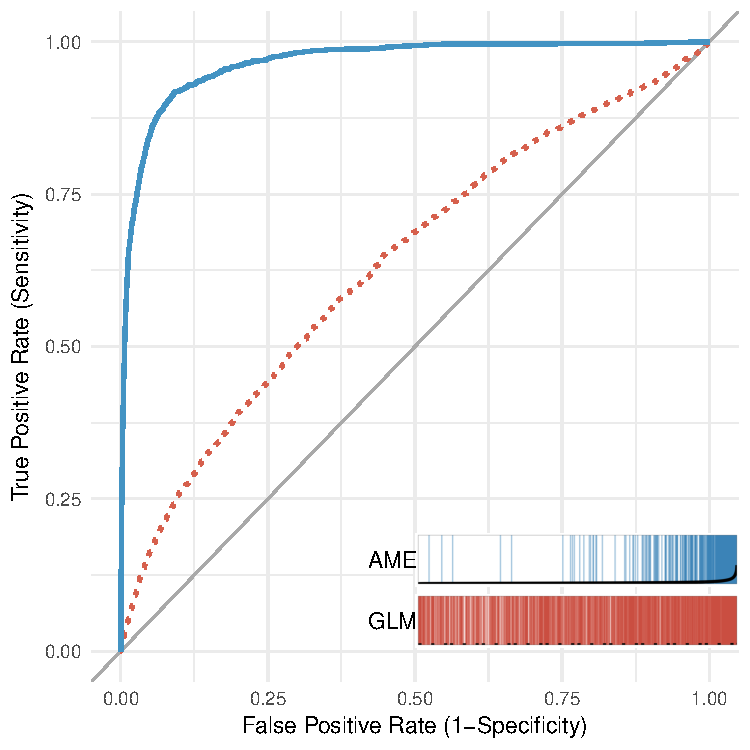
\includegraphics[width=.45\textwidth]{weeks_roc_outSample.pdf}}
%   \subfigure[Precision and Recall]{\label{fig:reitpr}\includegraphics[width=.45\textwidth]{weeks_pr_outSample.pdf}}
%   \caption{Assessments of out-of-sample predictive performance for Weeks (2012) using ROC curves and PR curves}
% \end{figure}
\FloatBarrier
\clearpage

\subsection*{Gibler (2017)}

Additional information for the Gibler (2017) re-estimation.

% latex table generated in R 4.0.3 by xtable 1.8-4 package
% Mon Jul 05 07:36:29 2021
\begin{table}[ht]
\centering
\begingroup\normalsize
\begin{tabular}{lcc}
 Variable & GLM (Logit) & AME \\ 
  \hline
\hline
(Intercept) & -5.826 & -4.056 \\ 
   & (0.366) & (0.168) \\ 
  Allied & 0.133 & 0.058 \\ 
   & (0.102) & (0.026) \\ 
  Joint Democracy & -0.527 & 0.03 \\ 
   & (0.099) & (0.023) \\ 
  Peace Years & -0.261 & -0.063 \\ 
   & (0.016) & (0.004) \\ 
  Spline 1 & -0.001 & 0.000 \\ 
   & (0.000) & (0.000) \\ 
  Spline 2 & 0.000 & 0.000 \\ 
   & (0.000) & (0.000) \\ 
  Spline 3 & 0.000 & 0.000 \\ 
   & (0.000) & (0.000) \\ 
  Contiguity & 2.427 & 0.594 \\ 
   & (0.196) & (0.028) \\ 
  Parity & -0.77 & 0.006 \\ 
   & (0.551) & (0.085) \\ 
  Parity at Entry Year & 2.034 & -0.221 \\ 
   & (0.617) & (0.084) \\ 
  Rivalry & 2.034 & 0.679 \\ 
   & (0.213) & (0.032) \\ 
   \hline
\hline
\end{tabular}
\endgroup
\caption{Parameter comparison for Gibler (2017). Standard errors in parentheses.} 
\label{tab:appendix_tableB3_coef}
\end{table}

\FloatBarrier

% \begin{figure}
% 	\centering
% 	\subfigure[AUC]{\label{fig:giblerroc}\includegraphics[width=.45\textwidth]{gibler_roc_outSample.pdf}}
% 	\subfigure[Precision and Recall]{\label{fig:giblerpr}\includegraphics[width=.45\textwidth]{gibler_pr_outSample.pdf}}
% 	\caption{Assessments of out-of-sample predictive performance for Gibler (2017) using ROC curves, PR curves, and separation plots.}
% \end{figure}
\FloatBarrier
\clearpage


\section{Additional Simulations: Non-Linear Data}

Aronow et al note that ``fitting a linear approximation to mildly non-linear data'' can be problematic for dyadic random effect models. We agree on the importance of testing this in the context of the simulation that we posed in the paper. Aronow et al incorporate non-linear misspecification by adding in squared version of the key dyadic homophily variable to the DGP for their simulations: $Y_{i,j} = \beta_{0} + \beta_{1} X_{i,j} + \beta_{2} X_{i,j}^{2} + \epsilon_{i,j}$. Here $X$ is their representation of homophily and is considered observed, while $X^{2}$ is their check for robustness to misspecification and is unobserved. We incorporate the same type of misspecification into our probit simulation setup: $Z_{i,j} =  \mu + \beta X_{i,j} + \gamma W_{i,j} + \epsilon_{i,j}$, where $W$ now instead of being drawn from a separate normal distribution is just the squared version of $X$. For the simulation we set values of $\mu$, $\beta$, and $\gamma$ to -2, 1, and 1, respectively. Results are shown below in Figures~\ref{fig:ameBias_asa} and \ref{fig:ameCalib_asa} below. As in the paper, along the x-axis we implement a standard model that does not take any steps to account for dependencies, AME, and the Oracle model, and as in the paper we find that the AME approach provides a number of benefits in terms of bias and coverage over the standard approach of not dealing with dependencies.

\begin{figure}[ht]
	\centering
	\caption{Regression parameter estimates for the standard, AME, and oracle models from 1,000 simulations. Summary statistics are presented through a traditional box plot, and the estimates from each simulation are visualized as well as points.}
	\label{fig:ameBias_asa}
	\includegraphics[width=1\textwidth]{graphics/appendix_figureC1.pdf} \\
\end{figure}

\begin{figure}[ht]
	\centering
	\caption{Proportion of times the true value fell within the estimated 95\% confidence interval for the standard, AME, and oracle models from 1,000 simulations.}
	\label{fig:ameCalib_asa}
	\includegraphics[width=1\textwidth]{graphics/appendix_figureC2.pdf} \\
\end{figure}

\FloatBarrier
\clearpage

\section{Additional Simulations: Correlation with Omitted Variable}

Estimation certainly gets more challenging when the omitted variable is correlated with the observed variable. In the case of normal linear regression, we can show that in general a regression coefficient is unbiased for its ``unconditional effect'', which is the direct effect plus something related to the direct effects of any omitted variables that it is correlated with. For example, suppose in our simulation setup $X_{i,j}$ is correlated with $W_{i,j}$ via the relation $W_{i,j} = \alpha X_{i,j} + e_{i,j}$. Then:

\begin{align*}
  Y_{i,j} & = \mu + \beta X_{i,j} + \gamma W_{i,j} + \epsilon_{i,j} \\
  &= \mu + (\gamma \alpha+\beta ) X_{i,j} + (\gamma Z_{i,j} + \epsilon_{i,j})  \\
  &= \mu + \tilde \beta X_{i,j} + \tilde \epsilon_{i,j}
\end{align*}

The naive model is in some sense still ``correct'' as it is an unbiased estimator of the unconditional (direct plus indirect) effect $\gamma\alpha + \beta$ of $X$ on $Y$. However, there is no way to eliminate this extra bias without making further assumptions about the nature of the omitted variable. Additonally, in the binary case with the probit setup, other sources of bias get introduced as well because of the nonlinearity of the population moments as a function of the parameters. An interesting question is whether or not we can reduce the bias in the network setting by assuming the omitted variable $w_{i,j}$ is the product of latent node-specific factors. An idea related to this is discussed in \citet{minhas:etal:2017:arxiv}.

For now though to show the amount of bias that gets introduced into our setup when $X$ and $W$ are correlated we repeat our simulation exercise but induce varying levels of correlation between $X$ and $W$. Results with $X$ and $W$ correlated at 0.4 and then 0.7 are shown below, respectively.

\begin{figure}[ht]
\caption{Regression parameter estimates for the standard, AME, and oracle models from 1,000 simulations. Summary statistics are presented through a traditional box plot, and the estimates from each simulation are visualized as well as points. $X$ and $W$ are correlated at 0.4 in this case.}
\label{fig:ameBias_corrMed}
\includegraphics[width=1\textwidth]{graphics/appendix_figureD1a.pdf} \\
\end{figure}

\begin{figure}[ht]
\caption{Regression parameter estimates for the standard, AME, and oracle models from 1,000 simulations. Summary statistics are presented through a traditional box plot, and the estimates from each simulation are visualized as well as points. $X$ and $W$ are correlated at 0.7 in this case.}
\label{fig:ameBias_corrHi}
\includegraphics[width=1\textwidth]{graphics/appendix_figureD1b.pdf} \\
\end{figure}

\FloatBarrier
\clearpage

\section{AME Tutorial}

Using the AMEN function requires formatting data into a particular structure. The primary distinction in data formatting is whether the outcome of interest represents a directed or undirected network.

If undirected, the AMEN function has three main inputs:

\begin{itemize}[noitemsep,nolistsep]
    \item Y: a $T$ length \textbf{list} of $n\times n$ adjacency matrices, where $T$ = number of years in the dataset and $n$ = number of nodes in the network.
    \begin{itemize}
      \item An adjacency matrix describes relationships between nodes in a particular year of data. For example, in an adjacency matrix of interstate MIDs, row $i$ and column $j$ takes a value of '1' if country $i$ and country $j$ had a MID in that year, and '0' otherwise. The diagonal in the adjacency matrix is typically missing. Y is a list of these adjacency matrices for the outcome variable, where each element in the list is a different year of data.
    \end{itemize}
    \item Xdyad: a $T$ length \textbf{list} of $n\times n\times p$ arrays, where $p$ = number of dyadic covariates in dataset.
    \begin{itemize}
      \item An array is a data object in R that contains a series of 'stacked' matrices for each year of data. An array of dimension (2, 3, 4), for example, contains 4 rectangular matrices each with 2 rows and 3 columns. Each matrix in the array describes the relationship between nodes with respect to some covariate. For example, for interstate alliances, row $i$ and column $j$ takes a value of '1' if country $i$ and country $j$ had an alliance in that year, and '0' otherwise. An array contains a matrix of this kind for each covariate going into the model. Xdyad is a list of these arrays, where each element in the list is a different year of data.
    \end{itemize}
    \item Xrow: a $T$ length \textbf{list} of $n\times p$ matrices, where $p$ = number of monadic (nodal) covariates in dataset.
    \begin{itemize}
      \item Each matrix in Xrow has the nodes running down the rows and the covariates in the dataset running along the columns. An entry in the matrix captures the value that a node takes on for each covariate in a given year. For example, if column $j$ is GDP per capita and column $k$ is population, then row $i$, column $j$ measures country $i$'s GDP per capita and row $i$, column $k$ measures country $i$'s population in a given year. Xrow is a list of these matrices, where each element in the list is a different year of data.
    \end{itemize}
\end{itemize}

If directed, AMEN further requires:

\begin{itemize}[noitemsep,nolistsep]
    \item Xrow: a $T$ length list of $n\times p$ matrices, where $p$ = number of sender (nodal) covariates in dataset.
    \begin{itemize}
      \item Xrow here is nearly identical to the undirected case. The only difference is that rather than each matrix containing covariate data on all nodes, in the directed context each matrix only contains data on the nodes that are acting as senders in that particular year. Using interstate MIDs as an example, if in 1983 only two countries initiated MIDs, Xrow would only contain data for those two countries (i.e., Xrow would only have two rows).
    \end{itemize}
    \item Xcol: a $T$ length list of $n\times p$ matrices, where $p$ = number of receiver (nodal) covariates in dataset.
    \begin{itemize}
      \item Xcol here is nearly identical to Xrow, except each matrix contains data on receiver nodes, not sender nodes. Using interstate MIDs as an example, if in 1983 only two countries had MIDs initiated against them, Xcol would only contain data for those two countries (i.e., Xcol would only have two rows).
    \end{itemize}
\end{itemize}

Beyond the data inputs, the AMEN function requires additional specification:

\begin{itemize}
    \item model: how to model the outcome variable, e.g., `logit'
    \item symmetric: whether the input network is symmetric
    \item intercept: whether to estimate an intercept
    \item nscan: number of iterations of the Markov chain
    \item burn: burn-in period
    \item odens: thinning interval
    \item R: dimension of the multiplicative effect (referred to as $K$ in the paper)
    \item gof: whether to calculate goodness of fit statistics
\end{itemize}

There is often little theoretical reason to choose a particular value of $\sf{R}$ (above). One strategy is to estimate models at different values of $\sf{R}$ and compare goodness of fit statistics across models. Given the computational time needed for parameter estimates to converge, parallelization strategies are recommended to speed up analysis. In addition, providing AMEN function with starting values, either dictated by theory, previous research, or previous runs can also help speed up convergence time.

The code below presents an example of an AME model running in parallel across 4 different levels of $\sf{R}$. Note also that the model is using starting values from a previous run, defined in \textit{startVals}.

\begin{lstlisting}[language=R]
# running in parallel varying k
imps = 10000 ; brn = 25000 ; ods = 10 ; latDims = 0:3

# Run amen in parallel
library(doParallel) ; library(foreach) ; cl=makeCluster(4) ; registerDoParallel(cl)
foreach(ii=1:length(latDims), .packages=c("amen")) %dopar% {

  # load previous model run
  load(prevModelFiles[ii])
  # extract start vals
  startVals0 = ameFit$'startVals'
  # dump rest
  rm(ameFit)

  ameFit = ame_repL(
    Y=yList,Xdyad=xDyadList,Xrow=NULL,Xcol=NULL,
    model="bin",symmetric=FALSE,intercept=TRUE,R=latDims[ii],
    nscan=imps, seed=1, burn=brn, odens=ods,
    plot=FALSE, print=FALSE, gof=TRUE, startVals=startVals0,
    periodicSave=TRUE )
  save(ameFit, file=paste0('model_k', latDims[ii],'_v2.rda') )
}
stopCluster(cl)
\end{lstlisting}



\end{document}
